\section{Introduction}

	Actin networks are remarkably dynamic and versatile and organize in a variety of cytoskeletal architectures to accomplish crucial cellular functions \cite{Banerjee2020}. For instance, isotropic thin actin gels form the cell cortex, which largely determines cell shape \cite{chugh2018} and motility in confined non-adherent environments \cite{blaser2006, Ruprecht:2015aa}. Polar structures at the edge of adherent cells, either forming filaments as in filopodia or sheets as in lamellipodia \cite{blanchoin2014}, enable cells to probe their environment and crawl on substrates. Nematic actin bundles, formed by anti-parallel fibers, conform a variety of contractile structures \cite{schwayer2016}, including the cytokinetic ring \cite{anne2016}, supra-cellular rings during wound healing \cite{martin1992} or development \cite{Krieg:2008aa}, subcellular bundle networks during cellularization \cite{dudin2019}, or stress fibers \cite{10.1242/jcs.236604,tojkander2012, tojkander2015}. Nematic bundles consist of highly aligned and densely packed actin filaments of mixed polarity inter-woven by a diversity of cross-linkers and whose assembly and maintenance depends on actin nucleators and regulators \cite{tojkander2012,blanchoin2014,schwayer2016,chugh2018,Banerjee2020}. Observations in cells and reconstituted systems show the essential role of myosin activity and of crosslinking proteins in the formation and maintenance of actin bundles \cite{chrzanowska1996, thoresen2011,strehle2011,laporte2012,chugh2018,lehtimaki2021}.
	
	Several studies emphasize the morphological, mechanical, dynamical, molecular and functional specificities of each of the families of actin bundles such as dorsal, transverse, and ventral stress fibers or contractile rings \cite{hotulainen2006,naumanen2008,tojkander2012,tojkander2015,doi:10.1091/mbc.E18-02-0106}. Nevertheless, observations across cell types also suggest that these nematic strands emerge as a result of self-organization of the active actomyosin gel. Suggestive of such an active self-organization, nematic fibers often form patterns with regular spacing, sometimes with families of fibers along orthogonal directions  \cite{tee2015, tojkander2015,wirshing2017, yolland2019, jalal2019,10.1242/jcs.236604}, dynamically fuse \cite{hotulainen2006,wirshing2017} and form a mechanically coherent network with the isotropic cortical network \cite{vignaud2021,lehtimaki2021}. Despite the self-organization of the actin cytoskeleton has been examined with active gel models in various contexts \cite{callan2013,kruse2004,hannezo2015},
	%, such as cell polarization \cite{callan2013}, the formation of asters \cite{kruse2004} or supracellular rings \cite{hannezo2015}, 
	the active self-organization of dense aligned nematic fibers and their dynamical interplay with a low-density, isotropic background network is not understood.

	To test the idea of physical self-organization of such nematic bundles, we develop here an active gel model accounting for nematic order in the spirit of \cite{salbreux2009,anne2016,julicher2018}. In agreement with the fact that nematic bundles require contractile activity, the transition from isotropic to nematic states is driven by active power input rather than by a more conventional density-dependent mechanism \cite{e2011}. Using linear stability analysis of the dynamical equations, we identify a distinct mechanism of pattern formation coupling density and nematic order variations. We further examine the fully nonlinear regime through numerical simulations, which establish the conditions for the self organization of an initially isotropic and uniform actin gel into dense nematic bundles and establish how key non-dimensional parameters affect the geometry and dynamics of bundle networks. Finally, we test the two key requirements for dense nematic bundle self-organization, namely the existence of active tension anisotropy and active forces conjugate to nematic order, using discrete network simulations. 	
    \begin{figure}[H]
		\centering
		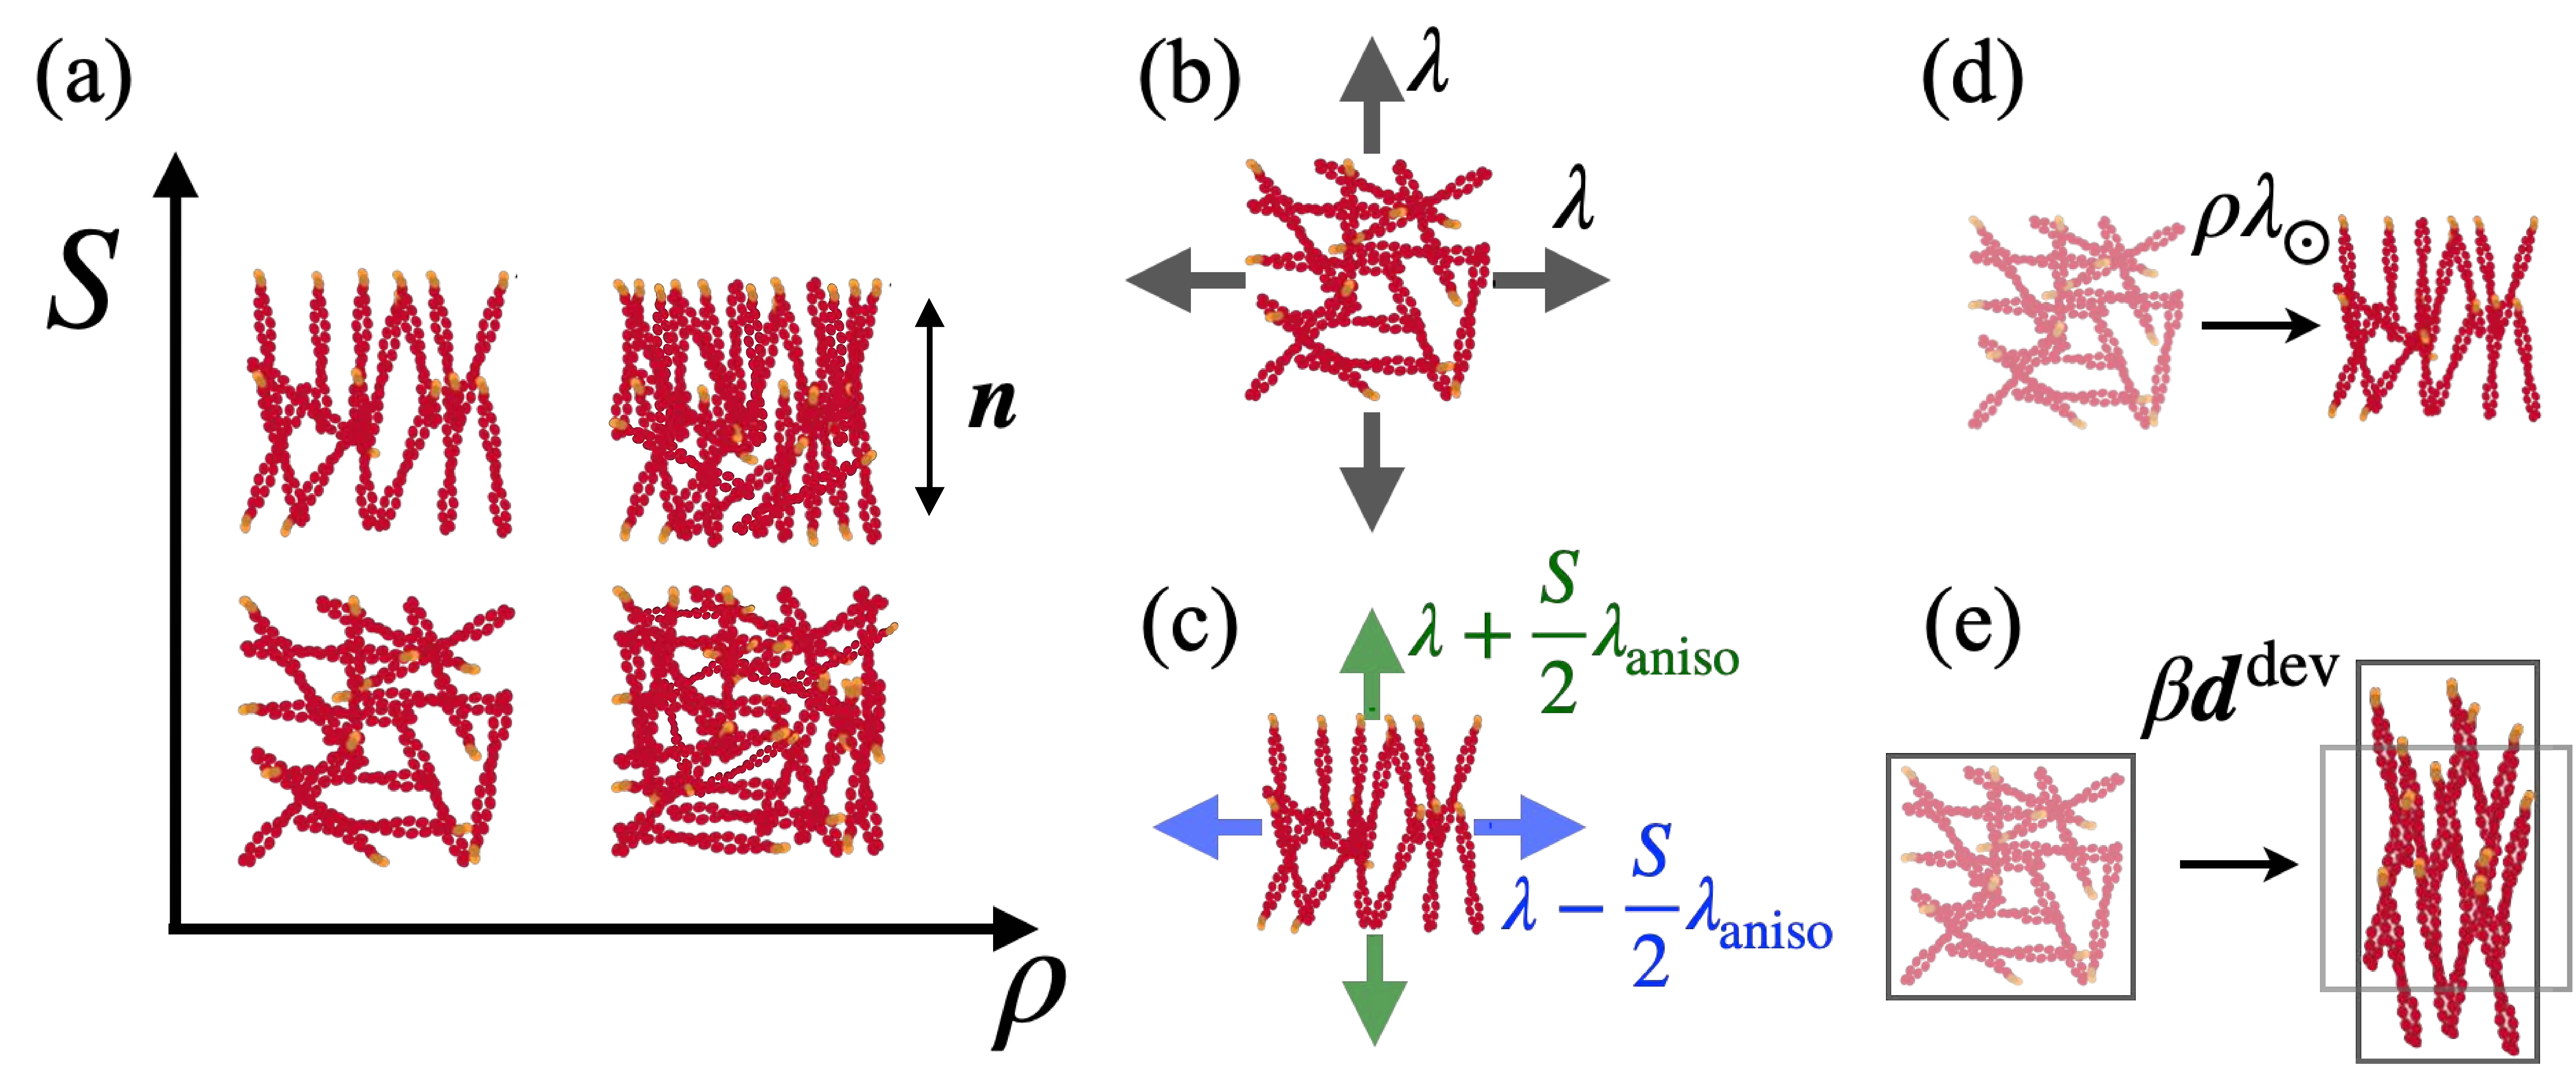
\includegraphics[width=0.7 \textwidth]{Figure_1.png}
		\caption{{\bf Key model ingredients}. (a) The local state of the system is defined by its density $\rho$ and by its orientational order quantified by the nematic parameter $S$ and by the nematic direction $\bm{n}$.  (b) Active tension is isotropic and given by parameter $\lambda$ when the network is isotropic ($S=0$), and (c) becomes anisotropic as $S$ increases as controlled by non-dimensional parameter $\kappa = \lambda_{\rm aniso}/\lambda$. Orientational order is driven by (d) active forces conjugate $S$ and characterized by parameter $\lambda_{\odot}$ and by (e) passive flow-induced alignment in the presence of deviatoric rate-of-deformation with coupling parameter $\beta$.}
		\label{fig4.1}
	\end{figure} 

	\section{Results}
	\noindent{\bf Theoretical model.}	As a coarse-grained description of a thin layer actin cytoskeleton, as in the cortex, we consider a nematic active gel in 2D. A number of active cellular and cytoskeletal systems have been modeled using nematic active liquid-crystal theory, including dense colonies of elongated cells or dense confined cytoskeletal gels \cite{giomi2014,duclos2017,kumar2018}. In such systems, crowding forces strong nematic order everywhere except at defects, which are generated by activity or required by topology. We argue that the porous actin cytoskeleton is not a nematic active liquid-crystal because it can adopt extended isotropic or low-order phases, and hence defects are not topologically required. Furthermore, the main mechanism driving nematic order is active contractility \cite{hotulainen2006}. Finally, liquid crystals are crowded and hence nearly incompressible, whereas actin gels develop large density variations.  We thus formulate an active gel model capable of accommodating large density variations and where nematic ordering is actively driven. 
	
	 At a given time $t$, the state of the system is described by the areal density of cytoskeletal material $\rho$ and by the network architecture quantified by the nematic order tensor $\bm{q}$, see Fig.~\ref{fig4.1}a. Assuming a fixed volumetric density $\rho_{\rm vol}$, $\rho$ can be interpreted as a cytoskeletal thickness $\rho/\rho_{\rm vol}$. The nematic tensor can be expressed as  $q_{ij} =S\left({n}_i n_j - \delta_{ij}/2 \right)$, where $\bm{n}$ is the average molecular alignment and $S=\sqrt{2   q_{ij}q_{ij}}$ the degree of local alignment about $\bm{n}$. We denote by $\bm{v}( \bm{x},t )$ the velocity field of the gel and by $\bm{d} = \frac{1}{2}(\nabla \bm{v}+ \nabla \bm{v}^T)$ and $\bm{w} = \frac{1}{2}(\nabla \bm{v}- \nabla \bm{v}^T)$ the rate-of-deformation and spin tensors. The rate of change of $\bm{q}$ relative to a frame that translates and locally rotates with the flow generated by $\bm{v}$ is given by the Jaumann derivative $\hat{\bm{q}} = \partial \bm{q} /\partial t + \bm{v} \cdot \nabla \bm{q}- \bm{w} \cdot \bm{q} +  \bm{q} \cdot \bm{w}$ \cite{de1993}.

Based on Onsager's variational formalism \cite{doi2011,arroyo2018}, we systematically derive the governing equations as detailed in Chapter~\ref{chap_2} and summarized next. According to this formalism, the dynamical equations of the active gel result from a competition between nematic free-energy release, dissipation and active power input subjected to mass balance. Because we consider a bi-periodic domain, we ignore here explicit boundary terms. 

Transport and turnover of the cortical material is described by 
\begin{equation} \label{eq_thick}
	\frac{\partial \rho }{\partial t} + \bm{\nabla} \cdot \left ( \rho \bm{v} \right) - D \Delta \rho + k_d(\rho-\rho_0)=0,
\end{equation}
where $D$ is an effective diffusivity, $\rho_0$ is the steady-state areal density and $k_d$ is the depolymerization rate. Balance of linear momentum takes the form
\begin{equation} \label{eq_lin_mom}
	\rho \gamma \bm{v} = \bm{\nabla} \cdot \bm{\sigma},
\end{equation}
where $\gamma>0$ models friction with a background medium and  $\bm{\sigma}$ is the Cauchy stress tensor, which in 2D has units of tension. We split it into symmetric and antisymmetric components as $\bm{\sigma} = \bm{\sigma}^{\rm s} + \bm{\sigma}^{\rm a}$. The symmetric component is given by
\begin{align}
	{\sigma}^{\rm s}_{ij} = & \rho \bigg\{  2\eta \left[ d_{ij} + d_{kk} \delta_{ij}\right]+ \beta  \hat{{q}}_{ij}  + {\sigma}^{\rm act}_{ij} - L q_{kl,i} q_{kl,j}  \bigg\},  \label{symm_stress} 
\end{align}
where $L>0$ is the Frank constant, $\eta>0$ is the shear viscosity, $\beta<0$ measures the dissipative coupling between nematic order and strain rate \cite{anne2016}, which here induces a stress proportional to changes in nematic tensor, and  ${\sigma}^{\rm act}_{ij}$ is the active tension resulting from expenditure of chemical energy in the gel. To model the dependence of contractility on network architecture \cite{Ennomani2016}, we assume ${\sigma}^{\rm act}_{ij} = \lambda \delta_{ij} + \lambda_{\rm aniso} q_{ij} = \lambda \left( \delta_{ij}  + \kappa q_{ij} \right)$ where $\kappa = \lambda_{\rm aniso}/\lambda$ measures the sign and strength of active tension anisotropy. When order is low ($S\approx 0$), active tension is isotropic, Fig.~\ref{fig4.1}b, whereas when order is high, active tension becomes anisotropic, Fig.~\ref{fig4.1}c, with active tension along the nematic direction reflecting the sliding of antiparallel fibers driven by myosin motors, and perpendicular to it reflecting the the out-of-equilibrium binding of bundling proteins or myosins \cite{harris2006,courson2010,blanchoin2014,schuppler2016,li2017,nandi2018,Ennomani2016,chen2020}. The antisymmetric part of the Cauchy stress, derived from balance of angular momentum, is purely elastic-nematic and given by ${\sigma}^{\rm a}_{ij} =  L \nabla_l \rho \left( \nabla_l q_{kj} q_{ik} - \nabla_l q_{ki} q_{jk} \right) + \rho L  \left( q_{ik}\Delta q_{jk}  -q_{jk}  \Delta q_{ik}  \right)$.

Balance of the generalized forces power-conjugate to $\hat{\bm{q}}$ also includes viscous, elastic-nematic and active contributions, and takes the form  
\begin{equation} \label{eq_nemat}
	\eta_{\text{rot}} \hat{\bm{q}} + \beta \bm{d}^{\rm dev} + (2a + b S^2)  \bm{q} - L \Delta \bm{q} - L  \nabla\bm{q} \cdot \frac{\nabla \rho}{\rho} - \rho \lambda_{\bigodot} \bm{q} = 0,
\end{equation}
where $\eta_{\text{rot}}$ is a nematic viscous coefficient, the second term models alignment induced by strain rate (Fig.~\ref{fig4.1}e) with the deviatoric part of the rate-of-deformation tensor given by $\bm{d}^{\rm dev} = \bm{d} - ({\rm tr}\,\bm{d}/2) \bm{I}$, and $a>0$ and $b>0$ are susceptibility coefficients. The last term is an active generalized force controlled by activity parameter $\lambda_{\odot}\ge 0$  tending to further align filaments (Fig.~\ref{fig4.1}d) \cite{anne2016}. This term is linear in $\rho$ because in the expansion $\bar{\lambda}_{\odot} + \rho \lambda_{\odot}$ the constant contribution $\bar{\lambda}_{\odot}$ can be subsumed by the susceptibility parameter $a$. Thus, the active term acts as a negative density-dependent susceptibility. When $c_0 =2a - \rho_0 \lambda_{\odot}<0$, the system can sustain a uniform quiescent state with $\rho(\bm{x},t) = \rho_0$, $\bm{v}(\bm{x},t) = 0$ and a  non-zero nematic tensor satisfying $S^2 = -c_0/b$. Even if $c_0>0$ and hence the uniform quiescent state is devoid of order,  pattern formation can induce density variations such that $2a - \rho \lambda_{\odot}$ becomes locally negative and actively favors local nematic order. The dissipative parameters in the model are constrained by Onsager's inequality, $2\eta \, \eta_{\text{rot}} - \beta^2 \geq 0$ (see Section~\ref{inequality}), which guarantees positive dissipation \cite{Onsager1931}.

By freezing an isotropic state, $S=0$, our model reduces to an orientation-independent active gel model, which develops periodic out-of-equilibrium patterns driven by self-reinforcing active flows sustained by turnover \cite{hannezo2015}. However, here the dynamics of orientational order, Eq.~(\ref{eq_nemat}), are coupled to the translational and density dynamics, Eqs.~(\ref{eq_thick},\ref{eq_lin_mom}), through $\beta$ and the term involving $\rho \lambda_{\odot}$, and conversely translational  dynamics, Eq.~(\ref{eq_lin_mom}), directly affect density dynamics, Eq.~(\ref{eq_thick}),  through $\bm{v}$ and depend on nematic order through the contributions to the stress tensor depending on $\kappa$, $\beta$ and $L$, Eq.~(\ref{symm_stress}). Hence, order affects translational and density dynamics. 

We readily identify the hydrodynamic length $\ell_s =\sqrt{\eta/\gamma}$, above which friction dominates over viscosity, the Damk\"olher length $\ell_D =\sqrt{D/k_d}$ above which reactions dominate over diffusion, and the nematic length $\ell_q=\sqrt{L/ \left | 2a - \lambda_{\odot} \, \rho_0 \right |}$. Non-dimensional analysis (see Section~\ref{appendix_1_sec_5}) reveals a set of non-dimensional groups that control the system behavior, namely the non-dimensional turnover rate $\bar{k}_d = \ell_s^2/\ell_D^2$, the  Frank constant $\bar{L} = L/(\eta D)$, the susceptibility parameters $\bar{a} = a/(\gamma D) and \bar{b} = b/(\gamma D)$, the drag coefficients $\bar{\eta}_{\rm rot} = {\eta}_{\rm rot}/\eta$ and $\bar{\beta} = \beta /\eta$, the nematic activity coefficient $\bar{\lambda}_\odot=\rho_0 \lambda_\odot / (\gamma D)$, and the active tension parameters $\bar{\lambda} = \lambda / (\gamma D)$ and $\kappa$.  The full list of material parameters for each figure and movie is given in Tables~\ref{defaulttable},~A.3 and justified in Section~\ref{appendix_1_sec_7}.


\medskip
\noindent{\bf Onset and nature of pattern formation.} To examine the role of nematic order in the emergence of various actin architectures, we performed linear stability analysis of our model particularized to 1D , see Sections~\ref{appendix_1_sec_4} and~\ref{appendix_1_sec_6}. The variables of the model are flow field along the $x-$direction $v(x,t)$, $\rho(x,t)$, and $q(x,t)$, where  $q>0\;(<0)$ corresponds to a nematic  orientation $\bm{n}$ parallel (perpendicular) to the $x-$axis. We first focused on the case $c_0=2a - \rho_0 \lambda_{\odot}>0$ to examine the loss of stability of a uniform, isotropic, and quiescent steady state ($\rho(x,t) = \rho_0$, $v(x,t) = 0$, $q(x,t)=0$) by increasing the master activity parameter $\lambda$ and identifying the most unstable modes. This allowed us to determine a threshold activity for pattern formation and the wavelength of the emerging pattern. Since the exact evaluation of such quantities requires solving nonlinear equations, we derived explicit expansions in the limit of small $L$ for the critical contractile activity 
\begin{align}
	\lambda_{\rm crit} \approx \lambda_{\rm crit,0} \left[1 - \frac{1}{2}\frac{\ell_s}{\ell_D}\left(1+  2\frac{\ell_s}{\ell_D}\right) \delta \right] + \mathcal{O}(\delta^2)
	\label{lam_c}
\end{align}
where $\lambda_{\rm crit,0} = (\sqrt{\gamma D} + 2 \sqrt{k_d\eta})^2 = \gamma D (1+2\sqrt{\ell_s/\ell_D})^2$ and $\delta = \gamma D \kappa \beta /(2\eta c_0)$, 
and for the the corresponding wavenumber
\begin{align}
	\nu_{\rm crit}^2 \approx \nu_{\rm crit,0}^2\left[1 + \frac{1}{8}\left(1 +  2\frac{\ell_s}{\ell_D}\right)^2 \delta \right] + \mathcal{O}(\delta^2), \label{nu_c}
\end{align}
where $\nu_{\rm crit,0}^2 = \left[k_d \gamma /(4\eta D)\right]^{1/2} = 1/({2\ell_s\ell_D})$. 

	
\begin{figure}
	\centering
	\includegraphics[width=0.9\textwidth]{Figure_2.pdf}
	\caption{{\bf Active formation of patterns coupling nematic order and density maintained by self-reinforcing flows and turnover.} (a) Dimensionless order parameter characterizing relative orientation of nematic direction and high-density bands defined by $\omega = {\ell_s^2}/{(\rho_0^2\vert A\vert)}\int_A \nabla\rho\cdot \boldsymbol{q} \nabla\rho~dS$ as a function of active tension anisotropy parameter $\kappa$, showing transition from states with nematic direction parallel to high-density structures ($\omega<0$), which we call fibrillar patterns, for $\kappa<0$ to states with nematic direction perpendicular to high-density structures  ($\omega>0$), which we call sarcomeric patterns, for $\kappa>0$. (b) Map of density, nematic order $S$, nematic direction (red segments) and flow field (green arrows) for quasi-steady fibrillar (I), sarcomeric (III) patterns, and for a transition pattern of high density droplets with high nematic order (II) corresponding to isotropic active tension (small $\kappa$). (c) These quasi-steady states are out-of-equilibrium and maintained by self-reinforcing flows and turnover.}
	\label{fig4.2}
\end{figure} 



When  $\kappa = 0$ or $\beta =0$, and hence $\delta = 0$, we recover the predictions of an active gel model not accounting for network architecture \cite{hannezo2015}, $\lambda_{\rm crit} = \lambda_{\rm crit,0}$ and $\nu_{\rm crit} = \nu_{\rm crit,0}$. However,  active tension anisotropy ($\kappa \ne 0$) and flow-induced alignment ($\beta <0$) fundamentally change the nature of pattern formation. Nematic order introduces  quantitative changes in critical tension and wavenumber, which depend on the ratio of hydrodynamic and Damk\"olher lengths and on the strength and sign of nematic coupling and can be very significant depending on the parameter regime. The nematic corrections increase as $c_0 \rightarrow 0$, close to the point where the uniform quiescent state develops spontaneous order. We thus studied separately the regime $0<c_0 \ll 1$ (details in Section~\ref{appendix_1_sec_6}), finding analogous expansions for the critical tension and wavenumber in terms of $\delta = \gamma D \kappa \beta /(2\eta L)$. Interestingly, Eq.~(\ref{lam_c}) shows that the activity threshold is reduced, and hence pattern formation facilitated, when $\kappa<0$, i.e. when active tension is larger perpendicular to the nematic direction. Besides these quantitative changes in critical tension and wavenumber, the present model predicts that the dynamical modes with self-reinforcing flows create patterns where high density co-localizes with high nematic order.
%\MAB{Our analysis predicts that the sign of $q(x,t)$ in regions of high density coincides with that of $\kappa$, i.e.~filaments align along/perpendicular to the $x-$direction when active tension is larger along/perpendicular to the nematic direction. [Please check this]}



To test the validity of this analysis and further understand the system beyond the onset of pattern formation, we performed fully non-linear finite element simulations (see Chapter~\ref{chap_3}) in a periodic 2D domain. In these simulations, we increased the activity parameter $\lambda$ beyond the instability starting from a quiescent uniform state. We found that the linear stability analysis very accurately predicts the activity thresholds and pattern wave-numbers within two percent across a wide range of parameters. In the nonlinear regime, the exponentially-growing instabilities eventually reach out-of-equilibrium quasi-steady-state patterns maintained by turnover and by self-reinforcing flows towards regularly-spaced regions of high density surrounded by a low density matrix. 

In the absence of nematic coupling ($\beta = \kappa = \lambda_\odot = 0$), these high density domains are droplets arranged in a regular hexagonal lattice with $S=0$ throughout the domain, \href{https://github.com/waleedmirzaPhD/movies_thesis.git}{Movie~4.1}, see Appendix~\ref{appendix_3}. In contrast, for a generic parameter set with finite $\beta$, $\kappa$ and  $\lambda_\odot$,  high density domains adopt elongated configurations or bands where order is high, surrounded by a low density and low order matrix, Fig.~\ref{fig4.2}b and \href{https://github.com/waleedmirzaPhD/movies_thesis.git}{Movie~4.2}, see Appendix~\ref{appendix_3}. Thus, the shape and internal architecture of dense phases are qualitatively modified by the nematic coupling.


Our simulations show that self-reinforcing flows develop along the direction of largest active tension, and consequently the pattern architecture changes qualitatively depending on the sign of $\kappa$, Fig.~\ref{fig4.2}c. For $\kappa<0$, the system self-organizes into high-density and high-order bands, where nematic direction is parallel to their axis, in what we call  \emph{fibrillar pattern}, Fig.~\ref{fig4.2}b(I). Instead, for $\kappa>0$ nematic order is perpendicular to the axis of the bands, in what we call \emph{sarcomeric pattern}, Fig.~\ref{fig4.2}b(III). To systematically study the effect of active tension anisotropy, we varied $\kappa$ between -0.8 and 0.8 while keeping all other non-dimensional groups fixed and  setting $\lambda$ to be 1.3 times the critical activity. We defined the order parameter $\omega$,  Fig.~\ref{fig4.2}a, allowing us to distinguish between sarcomeric ($\omega>0$) and fibrillar ($\omega<0$) organizations. We found a transition regime between the fibrillar and sarcomeric regimes, for small $\vert\kappa\vert$, in which elongated high-density and high-order domains fragment into  nematic droplets or tactoids, Fig.~\ref{fig4.2}b(II), which have been observed in reconstituted systems \cite{weirich2017,weirich2019}.

Our results for $\kappa<0$, leading to self-organized dense nematic fibrillar patterns from an isotropic low-density network, are in agreement with evidence suggesting that stress fibers can assemble from the actin cortex without the involvement of stress fiber precursors or actin polymerization at focal adhesions \cite{lehtimaki2021}, and with the spontaneous organization of reconstituted actin networks following addition of bundling agents \cite{deshpande2015}. They also agree with observations showing that actin bundles form a mechanical continuum with the surrounding sparse and isotropic cortex \cite{vignaud2021}. The morphology and patterning dynamics of our fibrillar pattern is strikingly reminiscent of actin microridges, formed at the apical surfaces of 
mucosal epithelial cells \cite{https://doi.org/10.1002/ar.23965,10.1083/jcb.201904144}, Fig.~\ref{chap_1_fig_777}. Finally, we also note the similarity in terms of density and nematic architecture between our fibrillar patterns and those emerging in other active systems through different mechanisms of self-organization, including polar motile filaments \cite{doi:10.1126/science.aao5434,Denk:2020vm} or mean-field models of dry mixtures of microtubules and motors \cite{C9SM00558G}. 

\medskip
\noindent{\bf Requirements for fibrilar and sarcomeric patterns.} At linear order, our theory shows that the distinctly nematic self-organization requires both flow-induced alignment ($\beta$) and active tension anisotropy ($\kappa$), whereas no condition is required on nematic activity ($\lambda_\odot$). We performed further simulations to establish the requirements for fibrillar and sarcomeric active patterning in the nonlinear regime. In contrast with the linear order prediction,both  sarcomeric and fibrilar patterns readily form for $\beta=0$ and finite $\kappa$, yet a finite value of $\beta$ enhances fibrillar formation, leading to longer and more stable dense bands, and hinders sarcomeric organization, \href{https://github.com/waleedmirzaPhD/movies_thesis.git}{Movie~4.3}, see Appendix~\ref{appendix_3}. This behavior is expected since the velocity gradients of the self-reinforcing flows tend to align filaments parallel to high-density bands due to the term $\beta \bm{d}^{\rm dev}$ in Eq.~(\ref{eq_nemat}). 

\begin{figure}
	\centering
	\includegraphics[width=0.99\textwidth]{Figure_3s.pdf}
	\caption{{\bf Control of nematic bundle pattern orientation, connectivity and dynamics.} \href{https://github.com/waleedmirzaPhD/movies_thesis.git}{Movie~4.5} in Appendix~\ref{appendix_3} shows the dynamics of each of the six conditions in this figure. (a) Effect of orientational bias. (I) A uniform isotropic cytoskeleton self-organizes into a labyrinth pattern with defects. (II) A slight initial network alignment ($S_0 =0.05$) orients bundles, which still loose stability, bend, and generate/anneal defects. (III) A small background anisotropic strain-rate efficiently orients nematic bundles. (b) Promoting mechanical interaction between bundles. (I) Dynamical pattern obtained by reducing friction, and thereby increasing non-dimensional susceptibility parameters, $\bar{\lambda}_\odot$ and $\bar{k}_d$. Blue circles indicate events of bundle tangential recombination, cyan symbols triple junctions and black lines events of bundle disassembly (II) Nearly static pattern obtained increasing $\bar{k}_d$, (III) which becomes highly dynamic by further increasing $\bar{k}_d$. Black polygons indicate events of aster/bundle collapse and blue lines events of bundle nucleation.}   
	\label{fig4.3}
\end{figure} 


The active nematic coefficient $\lambda_\odot$ does not affect the onset of pattern formation according to linear stability analysis, but should contribute to order condensation in high-density regions since it appears multiplied by $\rho$ in Eq.~(\ref{eq_nemat}). Indeed, our nonlinear simulations show that $\lambda_\odot=0$ leads to very different patterns without clear elongated structures and very mild nematic patterning, Fig.~\ref{supplem_fig_1}(a). Enhancing nematic patterning by considering the largest possible value of $\vert \beta \vert$ allowed by Onsager's inequality leads to elongated structures for $\kappa<0$, but rather than high-order co-localizing with high density, the nematic field develops domains with 90$^\circ$ angles between high- and low-density regions, Fig.~\ref{supplem_fig_1}(b), in an architecture enhanced by higher friction $\gamma$, Fig.~\ref{supplem_fig_1}(c). Thus, the architectures found for $\lambda_\odot=0$ and $\kappa<0$ are distinct from the fibrillar pattern described previously. Similarly, rather than sarcomeres, for $\lambda_\odot=0$, $\kappa>0$ and high $\vert \beta \vert$ we found patterns of nematic asters (high-density droplets with radial  nematic organization around them), Fig.~\ref{supplem_fig_1}(b,c). 


Together, these results show that active tension anisotropy ($\kappa\ne0$) and nematic activity ($\lambda_\odot\ne 0$) are necessary and sufficient for nematic self-organization into fibrilar or sarcomeric patterns, with flow-induced alignment ($\beta<0$) favoring fibrilar organization. 

\medskip	
\noindent{\bf Morphological and dynamical diversity of self-organized fibrillar patterns.} Given the morphological and dynamical diversity of nematic bundles in actin gels across cell types, geometric confinement, mechanical environment, or biological and pharmacological treatments \cite{yolland2019, jalal2019,dudin2019,gupta2015, xia2019, Verkhovsky1997}, we varied model parameters to examine the architectures predicted by our active gel model, focusing on $\kappa<0$. Significant changes in the effective parameters of our active gel model are reasonable since the active mechanical properties of actomyosin gels strongly depend on micro-architecture both in reconstituted systems and in cells \cite{Ennomani2016,chugh2017}.

We first focused on alignment and defects in fibrillar patterns, Fig.~\ref{fig4.2}b. Because the initial state of the system is isotropic but  fibrillar patterns are not, the process of self-organization leads labyrinth patterns with domains and defects. These defects can remain frozen in quasi-steady states, as in Fig.~\ref{fig4.3}a(I), or dynamically nucleate, reorganize and annihilate in a behavior akin to active turbulence \cite{alert2022}, which we observed for high activity beyond $\lambda_{\rm crit}$ or for high active tension anisotropy, \href{https://github.com/waleedmirzaPhD/movies_thesis.git}{Movie~4.4}, see Appendix~\ref{appendix_3}. 

To understand the differences in the out-of-equilibrium patterns depending on $\kappa$ leading to a secondary instability of nematic bundles, we quantified the stress tensor along and perpendicular to the fibrillar pattern, Fig.~\ref{supplem_fig_2}. 
In all cases $\kappa<0$, and hence active contractile tension is larger perpendicular to nematic bundles as required for their self-assembly. Competing with active tension, viscous tension is negative and larger perpendicular to the bundles. Hence, depending on their relative magnitude, total tension can be larger along or perpendicular to the bundles. We found that for stable fibrillar patterns ($\kappa = -0.2$), total tension is larger along bundles, consistent with their relative straightness and indicating that a large fraction of the active power perpendicular to the bundles is dissipated in the perpendicular self-reinforcing flows, and hence is not available to perform power at a mesoscale. Instead, for stronger active anisotropy ($\kappa = -0.8$) total tension along nematic bundles is smaller than perpendicular to them, Fig.~\ref{supplem_fig_2}(c), suggesting that secondary instability involving bundle wrinkling, defect nucleation and anihilation may be triggered by their viscous buckling \cite{PhysRevLett.109.064502}. 

We then wondered about the effect on pattern formation of an orientational bias, which physically may be caused by cytoskeletal flows, boundaries or directed polymerization \cite{hotulainen2006}. 
To analyze this, we considered  $c_0$ to be slightly negative, leading to the uniform and nematic steady state $\rho(x,t) = \rho_0$, $v(x,t) = 0$ and $q(x,t) = q_0 = \pm \frac{1}{2} \sqrt{-c_0/b}$. The linear stability analysis around this state and further nonlinear simulations show that the essential phenomenology of Eqs.~(\ref{lam_c},\ref{nu_c}) and Fig.~\ref{fig4.2} is not altered by the slight pre-existing order, see Section~\ref{qne0}. Now, pre-existing order directs pattern orientation, although at later times the nematic bundles also develop secondary active instabilities  leading to coordinated bending, defect nucleation and annihilation, Fig.~\ref{fig4.3}a(II) and \href{https://github.com/waleedmirzaPhD/movies_thesis.git}{Movie~4.5a(II)}, see Appendix~\ref{appendix_3}. Alternatively, we also tested that a small background anisotropic strain-rate is sufficient to produce well-oriented defect-free patterns aligned with the direction of elongation, Fig.~\ref{fig4.3}a(III) and  \href{https://github.com/waleedmirzaPhD/movies_thesis.git}{Movie~4.5a(III)}, see Appendix~\ref{appendix_3}. Such background strain-rates are expected in the heterogeneous actin flows of adherent cells. Thus, an anisotropic bias can orient and anneal nematic fibrillar patterns. These results agree with the two examples of actin patterning in Fig.~\ref{chap_1_fig_777},  showing how cell shape anisotropy \cite{DINWIDDIE2014404} and uniaxial cell stretch \cite{10.1083/jcb.201904144} guide the orientation of dense actin bundles.


Previous work on isotropic gels has shown that reducing friction triggers chaotic dynamics as the distance between high-density regions, $2\pi/\nu_{\rm crit}$, becomes comparable or smaller than the hydrodynamic length scale  \cite{hannezo2015}, thus enabling their hydrodynamical interaction. In a model devoid of orientational order, reducing friction is equivalent to increasing $\bar{k}_d$. In our present model, however, we can either reduce $\gamma$, which in non-dimensional terms means increasing $\bar{k}_d$, $\bar{a}$, $\bar{b}$ and $\bar{\lambda}_\odot$ in concert, or increase $\bar{k}_d$ while leaving all other non-dimensional parameters fixed. The first of these choices leads to highly dynamical networks with frequent nucleation, disappearance and recombination of wiggly nematic bundles, Fig.~\ref{fig4.3}b(I) and  \href{https://github.com/waleedmirzaPhD/movies_thesis.git}{Movie~4.5b}, see Appendix~\ref{appendix_3}. We note, however, that  now total tension along bundles is much larger than perpendicular to them, Fig.~\ref{supplem_fig_2}(d), and hence the secondary instability cannot be attributed to viscous buckling. Because of the large active nematic parameter, nematic condensation is very strong. In a common recombination event, neighboring bundles merge tangentially to minimize nematic distortion (blue circles), leading to the formation of two junctions where three bundles meet (cyan symbols). These events are also observed during the early stages of actin gel reorganization following addition of cross-linkers \cite{weirich2017}. Nematic activity  $\bar{\lambda}_\odot$ being large, these dense triple junctions have high order and also high nematic gradients. Thus, they are energetically unfavorable and short-lived through the disassembly of one of the bundle segments (solid/dashed black lines).  The second choice to favor mechanical interaction of bundles, increasing $\bar{k}_d$, leads to very different networks with high-density aster-like clusters interconnected by straight actin bundles. Because now $\bar{\lambda}_\odot$ is not particularly large, order is low at the core of these clusters, enabling high-valence networks where four bundles often meet at one cluster. For $\bar{k}_d=10$, the network is stable and nearly crystalline, Fig.~\ref{fig4.3}b(II), whereas for $\bar{k}_d=20$, it becomes highly dynamical with frequent collapse of polygonal cells by fusion of neighboring actin clusters and their attached bundles (black polygons) and nucleation of new bundles within the low-density domains (dashed/solid blue lines), Fig.~\ref{fig4.3}b(III) and  \href{https://github.com/waleedmirzaPhD/movies_thesis.git}{Movie~4.5b}, see Appendix~\ref{appendix_3}. This architecture and dynamics resemble those in adherent epithelial cells treated with epidermal growth factor \cite{jalal2019} and in mouse embryonic stem cells \cite{xia2019}.

In summary, our theory maps how effective parameters of the actin gel control the active self-organization of a uniform and isotropic gel into a pattern of high-density nematic bundles embedded in a low-density isotropic matrix, including the activity threshold, the bundle spacing, orientation, connectivity and dynamics. 

\medskip
\noindent{\bf Microscopic origin of $\kappa<0$ and $\lambda_\odot>0$ through discrete network simulations.} A somewhat counter-intuitive prediction of our model is that the self-organization of nematic bundles, the most prominent emerging organization in actin gels across cell types and length-scales, requires that active tension perpendicular to nematic orientation is larger than along this direction ($\kappa<0$), at least at the onset of pattern formation. %This is at odds with the notion that, once formed, these fibers can exert significant axial active tension. 
While our continuum hydrodynamical model can address mesoscopic conditions for self-organization, it cannot provide insight about the microscopic origin of effective activity parameters. To examine whether the conditions $\kappa<0$ and $\lambda_\odot>0$ for spontaneous formation of fibrillar patterns are plausible from a microscopic point of view, we performed discrete network simulations using Cytosim, an open source code for agent-based cytoskeletal simulations \cite{Nedelec2007}. 


\begin{figure}[t]
	\centering
	\includegraphics[width=0.8\textwidth]{Figure_4.pdf}
	\caption{{\bf Assessment of activity parameters $\kappa$ and $\lambda_\odot$ through discrete network simulations.} (a) Sketch of discrete network simulations in the setup with boundary anchors, allowing us to compute tension parallel and perpendicular to the nematic direction. (b) Typical time-signal from simulations for parallel and perpendicular tensions following addition of crosslinkers and motors (translucent lines) along with time average (solid lines) for isotropic and anisotropic networks. Tension is normalized by mean tension $\bar{\sigma} = (\sigma_{||}+\sigma_{\bot})/2$ computed from time-averages and time by the inverse of the turnover rate. (c) Mean tension as a function of network density for several nematic parameters $S_0$, where both quantities are normalized by their values for a reference density. With this normalization, we expect a linear dependence with slope $\lambda = 1$, Eq.~(\ref{mean_dev}), which closely follows our fit to simulation data (dashed line). Error bars span two standard deviations. (d) Deviatoric tension normalized by mean tension as a function of nematic order for different densities. The dashed line is a linear regression to simulation data. (e) Dynamics  of nematic order in a periodic network following addition of crosslinkers and motors for three initial values of nematic order. (f) Rate of change of nematic oder normalized by turnover rate as a function of initial nematic order at zero and finite temperature. }
	\label{fig4.4}
\end{figure} 

Addressing the self-organization of the actin cytoskeleton at mesoscales directly with discrete network simulations is very challenging due to the large range in time- and length-scales and the need to realistically model diffusion, network renewal, friction and gel hydrodynamics. Instead, we aimed at characterizing the out-of-equilibrium mechanical behavior of a representative volume element of the material with uniform mesoscopic properties. We performed 2D simulations in which semi-flexible filaments interact with cross-linkers and myosin motors, all of which undergo turnover and have a stoichiometry previously used to model the actin cytoskeleton \cite{Cortes2020}, Fig.~\ref{fig4.4}(a). See Section~\ref{appendix_1_sec_8} for a detailed description of the simulation protocol. Briefly, we modified Cytosim to account for average orientational order in the simulation box, which we evaluated as a sample average of orientations over the ensemble of segments composing the filaments. We further introduced a nematic energy penalty in the network allowing us to restrain average nematic order to a target value $S_0$.
% with unit vector $\bm{m}^I$ making up the filaments, ${q}^s_{ij}(\bm{X}) = (1/N)\sum_{I=1}^N \left[ {m}^I_i {m}^I_j - (1/2) \delta_{ij}\right]$. Here, $\bm{X}$ denotes the vector of particle positions defining the model. To control average orientation of the network, we selectively added to the system hamiltonian the following restraining energy \MAB{[CAN BE SHORTENED]}
%	\begin{align}
	%		E_S (\bm{X}) = \frac{\mathcal{K}_S}{2} \left\vert\bm{q}^s(\bm{X}) - \frac{S_0}{2}\left(\begin{array}{cc}-1 & 0  \\0 & 1\end{array}\right) \right\vert^2,
	%		\label{E_S}
	%	\end{align}
%	where $S_0$ is the target orientational order parameter, $\mathcal{K}_S$ controls the strength of the restraint, and nematic direction is along the $y-$axis. 

We first prepared a system consisting only of randomly oriented actin fibers, imposed the desired orientational order $S_0$ using the nematic penalty  and equilibrated the system. In a first set of simulations, once $S_0$ was reached, we deactivated the nematic penalty and added cross-linkers and myosins, driving the system out-of-equilibrium. The free contraction of the system was prevented by the addition of anchors at the boundary of the representative volume element, which also allowed us to compute anchor forces and hence estimate the effective active tension along the nematic direction $\sigma_{||} = \sigma_{ij} n_i n_j$ and perpendicular to it, $\sigma_{\bot}=\sigma_{ij} m_i m_j$ with $n_im_i = 0$ and $m_im_i = 1$, Fig.~\ref{fig4.4}(a). 

Addition of crosslinkers and myosins leads to bundling of actin filaments at the microscale,  \href{https://github.com/waleedmirzaPhD/movies_thesis.git}{Movie~4.6} in Appendix~\ref{appendix_3}, distinct from the mesoscale fibrillar pattern formation emerging from the active gel model. It also leads to out-of-equilibrium tension as measured by the anchors. For an isotropic network ($S_0=0$), active tension is isotropic with $\sigma_{||}\approx\sigma_{\bot}$. For an anisotropic network, however, we found that tension becomes anisotropic with $\sigma_{\bot}>\sigma_{||}$, Fig.~\ref{fig4.4}(b). 

We systematically characterized this behavior varying initial orientational order and network density. According to our active gel model, Eq.~(\ref{symm_stress}), in the absence of nematic gradients and flow,  the tension components $\sigma_{||}$ and $\sigma_{\bot}$ satisfy the following relations in terms of mean and deviatoric tensions 
\begin{align}\label{mean_dev}
	\bar{\sigma} = (\sigma_{||}+\sigma_{\bot})/2 = \lambda \rho \;\;\;\mbox{and}\;\;\; (\sigma_{||}-\sigma_{\bot})/\bar{\sigma} = \kappa S.
\end{align}
Remarkably, our discrete network simulations closely followed these relations, Fig.~\ref{fig4.4}(c,d), which allowed us to estimate $\kappa \approx -1.6$. We perturbed selected parameters of the discrete network model and found that this behavior with $\kappa<0$ was general for relatively fast turnover rates of cross-linkers and myosins.
%We found that this behavior, which leads according to our active gel model to the formation fibrillar patterns, was rather general but required relatively fast turnover rates for cross-linkers and myosins, suggesting that cells can control the sign and magnitude of $\kappa$ by tuning the dynamics of cytoskeletal components. 

We then wondered if the discrete network simulations could provide evidence for the orientational activity parameter in our theory, $\rho \lambda_{\odot}$. For a uniform system with nematic order along a given direction and ignoring the susceptibility parameter $b$, Eq.~(\ref{eq_nemat}) becomes
\begin{align}
	\eta_{\rm rot}\dot{S} + (2a-\rho \lambda_{\odot})S + \mathcal{K}_S(S-S_0) = 0,
	\label{S_dyn}
\end{align}
where $\eta_{\rm rot}$ is the viscous drag of the filaments in the discrete network simulations, $a>0$ the entropic tendency of the model to return to isotropy, $\rho \lambda_{\odot}$ the active forcing of nematic order resulting from cross-linkers and motors, and the last term accounts for the effect of the nematic penalty with coefficient $\mathcal{K}_S$. As a first test of this model, we started from an isotropic and periodic network and tracked the athermal dynamics of $S$ under the action of the nematic penalty in the absence of anchors, cross-linkers and myosins. For  $ \lambda_{\odot} = 0$ and $a=0$, Eq.~(\ref{S_dyn}) predicts an exponential relaxation given by $S(t) = S_0 (1-e^{-K_St/\eta_{\rm rot}})$, which very closely matched the simulation data for different values of $S_0$ and for a single fitting parameter $\eta_{\rm rot}$, Fig.~\ref{supplem_fig_3}(III) and  \href{https://github.com/waleedmirzaPhD/movies_thesis.git}{Movie~4.7} in Appendix~\ref{appendix_3}. We then deactivated the nematic penalty and added cross-linkers and motors, but not anchors, to track unconstrained dynamics of nematic order starting from different values of $S_0$. In agreement with the notion of an active force driving nematic order, we found that $S(t)$ monotonically increased, Fig.~\ref{fig4.4}(e). More quantitatively, we tested the short-time prediction of Eq.~(\ref{S_dyn}), $\eta_{\rm rot}\dot{S} = (\rho \lambda_{\odot}-2a)S_0$, by plotting $\dot{S}$ as estimated from our simulations, as a function of $S_0$, Fig.~\ref{fig4.4}(e). We found a nearly linear relation with positive slope, hence providing evidence for an active generalized force driving order. In agreement with the theory, in the athermal limit, the tendency to actively increase order is faster as the entropic tendency to disorder is absent ($a=0$).  


In summary, discrete network cytoskeletal simulations provide a microscopic justification for two key ingredients of our active gel theory, namely that nematic order elicits (1) anisotropic active tensions, which can be larger perpendicular to the nematic direction ($\kappa<0$), and (2) active generalized forces driving further ordering. We do not rule out that in a different parameter regime of the network anisotropic tensions may be larger along the nematic direction ($\kappa>0$). For instance, once bundles are dense and maximally aligned, the ability of the  active nematic gel to perform active tension perpendicular to the nematic direction may saturate and, instead, the action of myosins along the nematic direction may be more effective. The regime studied here would assist the assembly of such dense nematic structures, which  would then become highly contractile. This rationale is qualitatively consistent with mean-field models of idealized filament-motor mixtures, where the sign of the active nematic coupling (here $\kappa$) depends on microscopic details \cite{C9SM00558G}. 


\section{Conclusions}

We have proposed a theory for the active self-organization of initially uniform and isotropic actin gels into various dense nematic architectures embedded in an isotropic matrix of low density. This model predicts a variety of emergent patterns involving asters, tactoids, sarcomeric bands, and more importantly nematic bundles, the most prominent nematic architecture across scales and cell types. We have characterized how the activity threshold, spacing, orientation, geometry, connectivity and dynamics of patterns of nematic bundles depends on effective active gel parameters. Because the active gel parameters at a mesoscale depend on the molecular architecture and dynamics of the network, our results portray actin gels as responsive and reconfigurable active materials that cells can finely regulate. Our theory identifies two key requirements on activity parameters for the the self-organization of patterns of nematic bundles, namely active tension anisotropy with larger tension perpendicular to the nematic direction and generalized active forces tending to increase nematic order. To substantiate these two requirements, we have used discrete network simulations of a representative volume element. which support the assumptions of our active gel model. 
Our work suggests further experimental and computational work to establish a more comprehensive mapping between microscopic architecture and dynamics and mesoscale active gel properties to bridge between molecular regulation and emergent cell-scale organization of the actin cytoskeleton.
	
